\chapter{Model}
\label{sec:model}
The model we used for this study, is called `Application of Research to Operations at Mesoscale' (AROME) and was developed by the ALADIN consortium  \cite{aladinhp}. At the `Zentralanstalt für Meteorologie und Geophysik' (ZAMG), the model has been operational since 2014, which means that it is not only used for research, but also for forecasts on a daily basis.  If not mentioned otherwise, all settings remained the same as for the operational configuration of the model at ZAMG.\\
As the name implies, AROME is a limited area model, written in Fortran. The version operationally used at ZAMG (C40T1) has a horizontal resolution of 2.5km on a 432-by-600 grid and 90 vertical layers. The highest layer is at a pressure level of 10hPa, which is the equivalent of approximately 25km. One time step is set to  60 seconds and the geographical model domain of central Europe is shown in several graphics in the following (e.g. Figure \ref{fig:stations} , \ref{fig:example-pert} ). It is a convection permitting and non-hydrostatic model \cite{gmd-2017-103}. Convection permitting means that ascending and descending convective currents are resolved, opposed to the strategy of simply parametrizing their effects, commonly done in global models with a lower resolution.\\
Since AROME is a LAM, it has to be nested in a model with a larger domain, to set its boundary values. At ZAMG the used model is the global European `Integrated Forecast System' (IFS), version C41R2, developed by the European Centre for Medium-Range Weather Forecasts (ECMWF) \cite{IFS}. The IFS model is operationally run with a 51 member ensemble at the ECMWF. ZAMG uses a subset of 16 members and the control member of the ECMWF-ensemble. \\
AROME was forked from the original ALADIN (Aire Limitée Adaptation Dynamique Développement International) model, which was developed by Météo-France. \\
Most parts of the code are contained in the common code package IAAA (IFS, ALADIN, AROME, ARPEGE) where AROME is a canonical configuration of the package \parencite{gmd-2017-103} and uses the so-called `MESO-NH' physics package \parencite{lafore1998p}.\\
For its dynamical core AROME uses a semi-implicit semi-Lagrangian scheme \parencite{gmd-2017-103,seity2011arome}. The Lagrangian and the Eulerian schemes are different methods for treating flow fields in continuum mechanics. A Lagrangian scheme describes a system by the movements of the parcels of the fluid. The counter-model of that, the Eulerian scheme, uses the change rates at specific locations to capture the dynamics of the field. In a semi-Lagrangian scheme an Eulerian grid is used and at each time step the trajectories that brought the parcels of the fluid to their current locations are calculated \cite{durran2010numerical}. The main reason why semi-Lagrangian schemes very common in NWP models is, because when combined with semi-implicit integration, they remain stable even for long time steps \cite{vincent}. 


\section{Spatial Discretization}
\begin{wrapfigure}{l}{0.4\textwidth}
    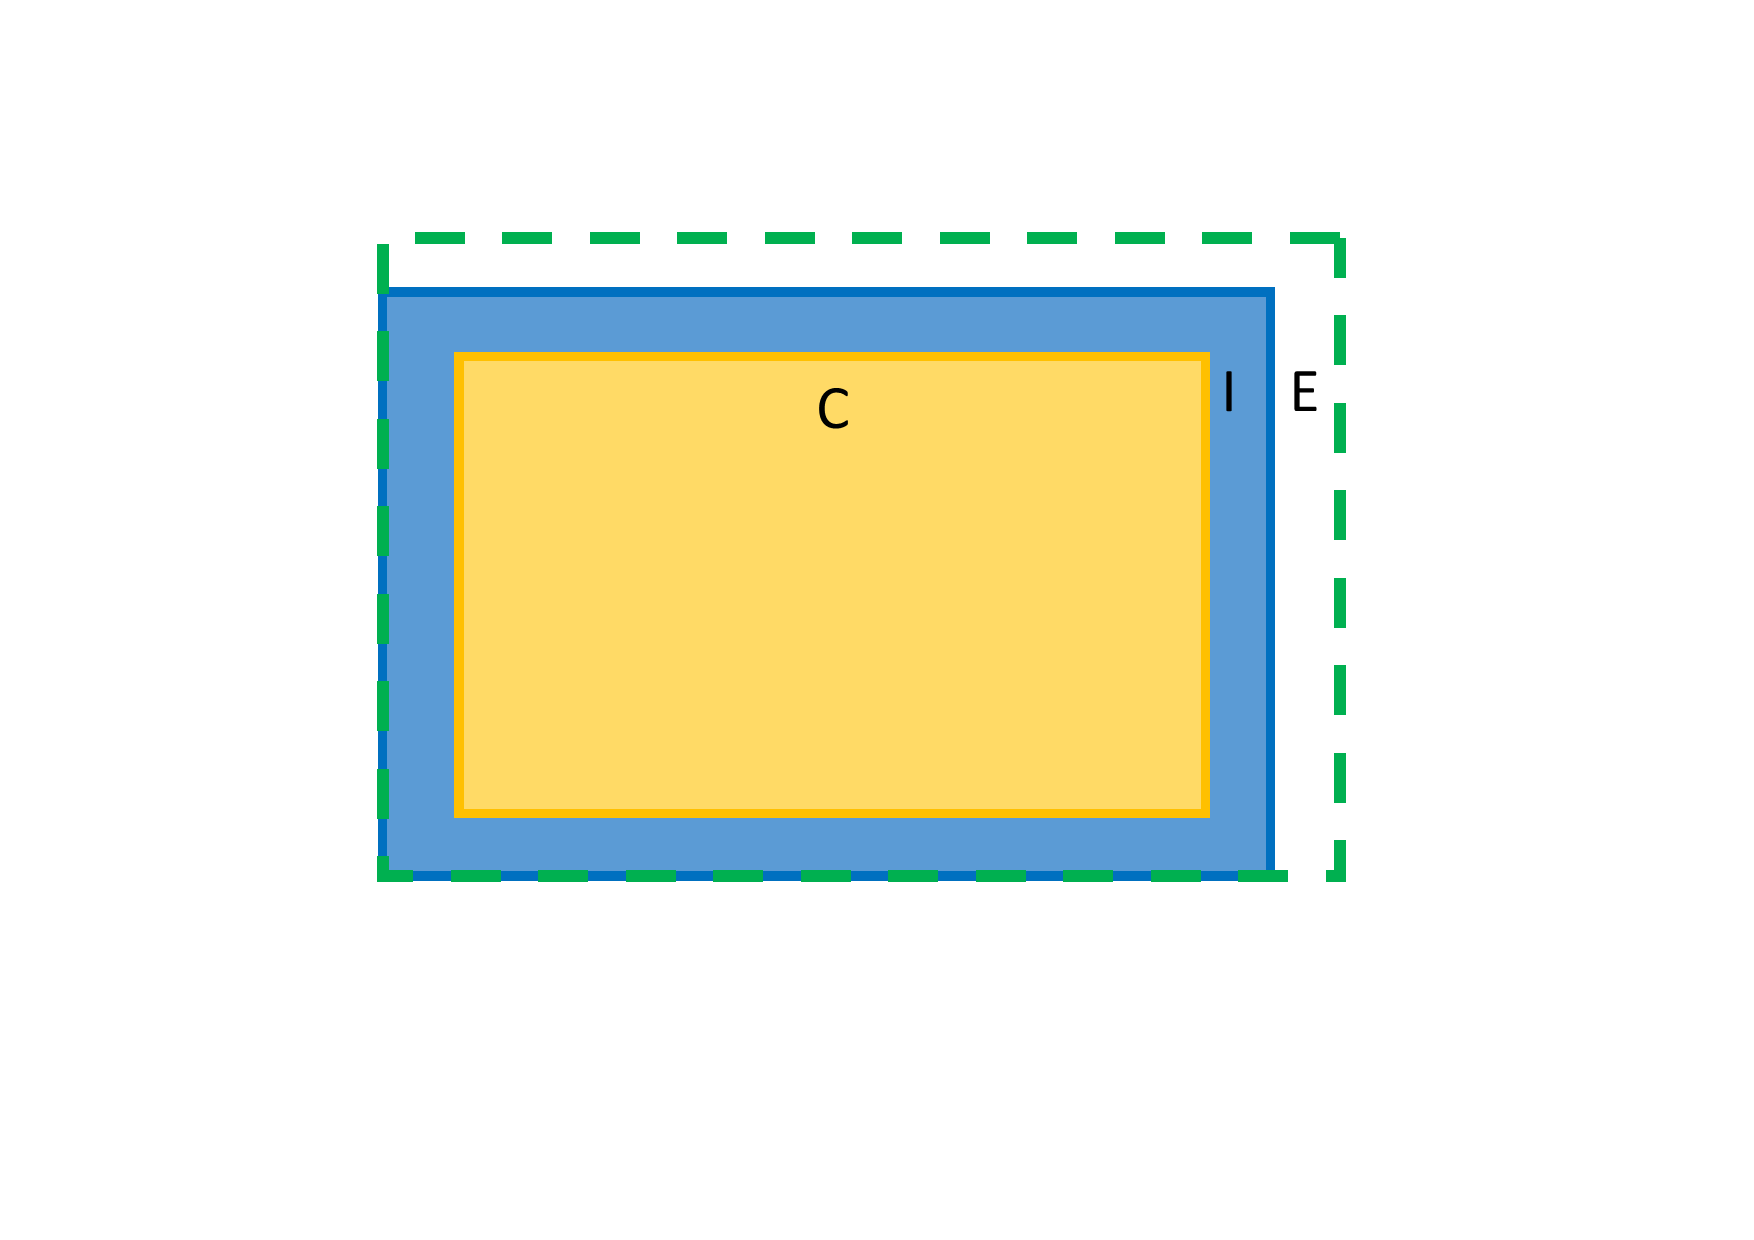
\includegraphics[trim={5cm 5cm  5cm  4cm },clip,
     width=0.9\linewidth] {graphics/Zones.png}
    \caption[Zones in AROME's Computational Domain]{Different Zones in AROME model domain: C - Central Zone, I - Intermediate Zone, E - Extension Zone \parencite{gmd-2017-103}}
    \label{fig:zones}
\end{wrapfigure}The AROME Model mainly uses spectral representations of the fields, with the exception of the grid point representation of humidity. Each time, fields of different types need to interact, a Fast Fourier Transformation (FFT) is performed. \\
The spectral horizontal discretization is a bi-Fourier spectral representation with elliptical truncation on a conical Lambert-projection, as illustrated in Figure \ref{fig:lambert}. The vertical discretization uses finite differences and finite elements \parencite{gmd-2017-103, meteofrance}.  
\\
Due to the bi-Fourier spectral representation, different zones (as shown in Figure \ref{fig:zones}) had to be introduced in the model.
The outermost zone E is called extension zone and is the actual computational domain of the spectral method. 
Because of the periodic nature of the Fourier Series the computational domain describes a torus. Consequently, it can never be congruent with the geographical LAM domain. To resolve this issue, the corresponding geographical domain is a cut-out of the extension zone to avoid physically nonsensical periodic values at the edges of the domain.
In the Intermediate Zone I the boundary conditions from the global model get sourced in.
Only in the Central Zone C can the physics and dynamics evolve completely freely. This zone can be seen as the equivalent of the geographical domain \cite{gmd-2017-103}.\\
The vertical coordinate is a hybrid pressure terrain-following coordinate. It is preferred over a simple pressure coordinate, because as illustrated in Figure \ref{fig:coordinates}, geographical barriers like mountains are considered.
\begin{figure}[H]
    \centering
    \begin{subfigure}{0.45\textwidth}
    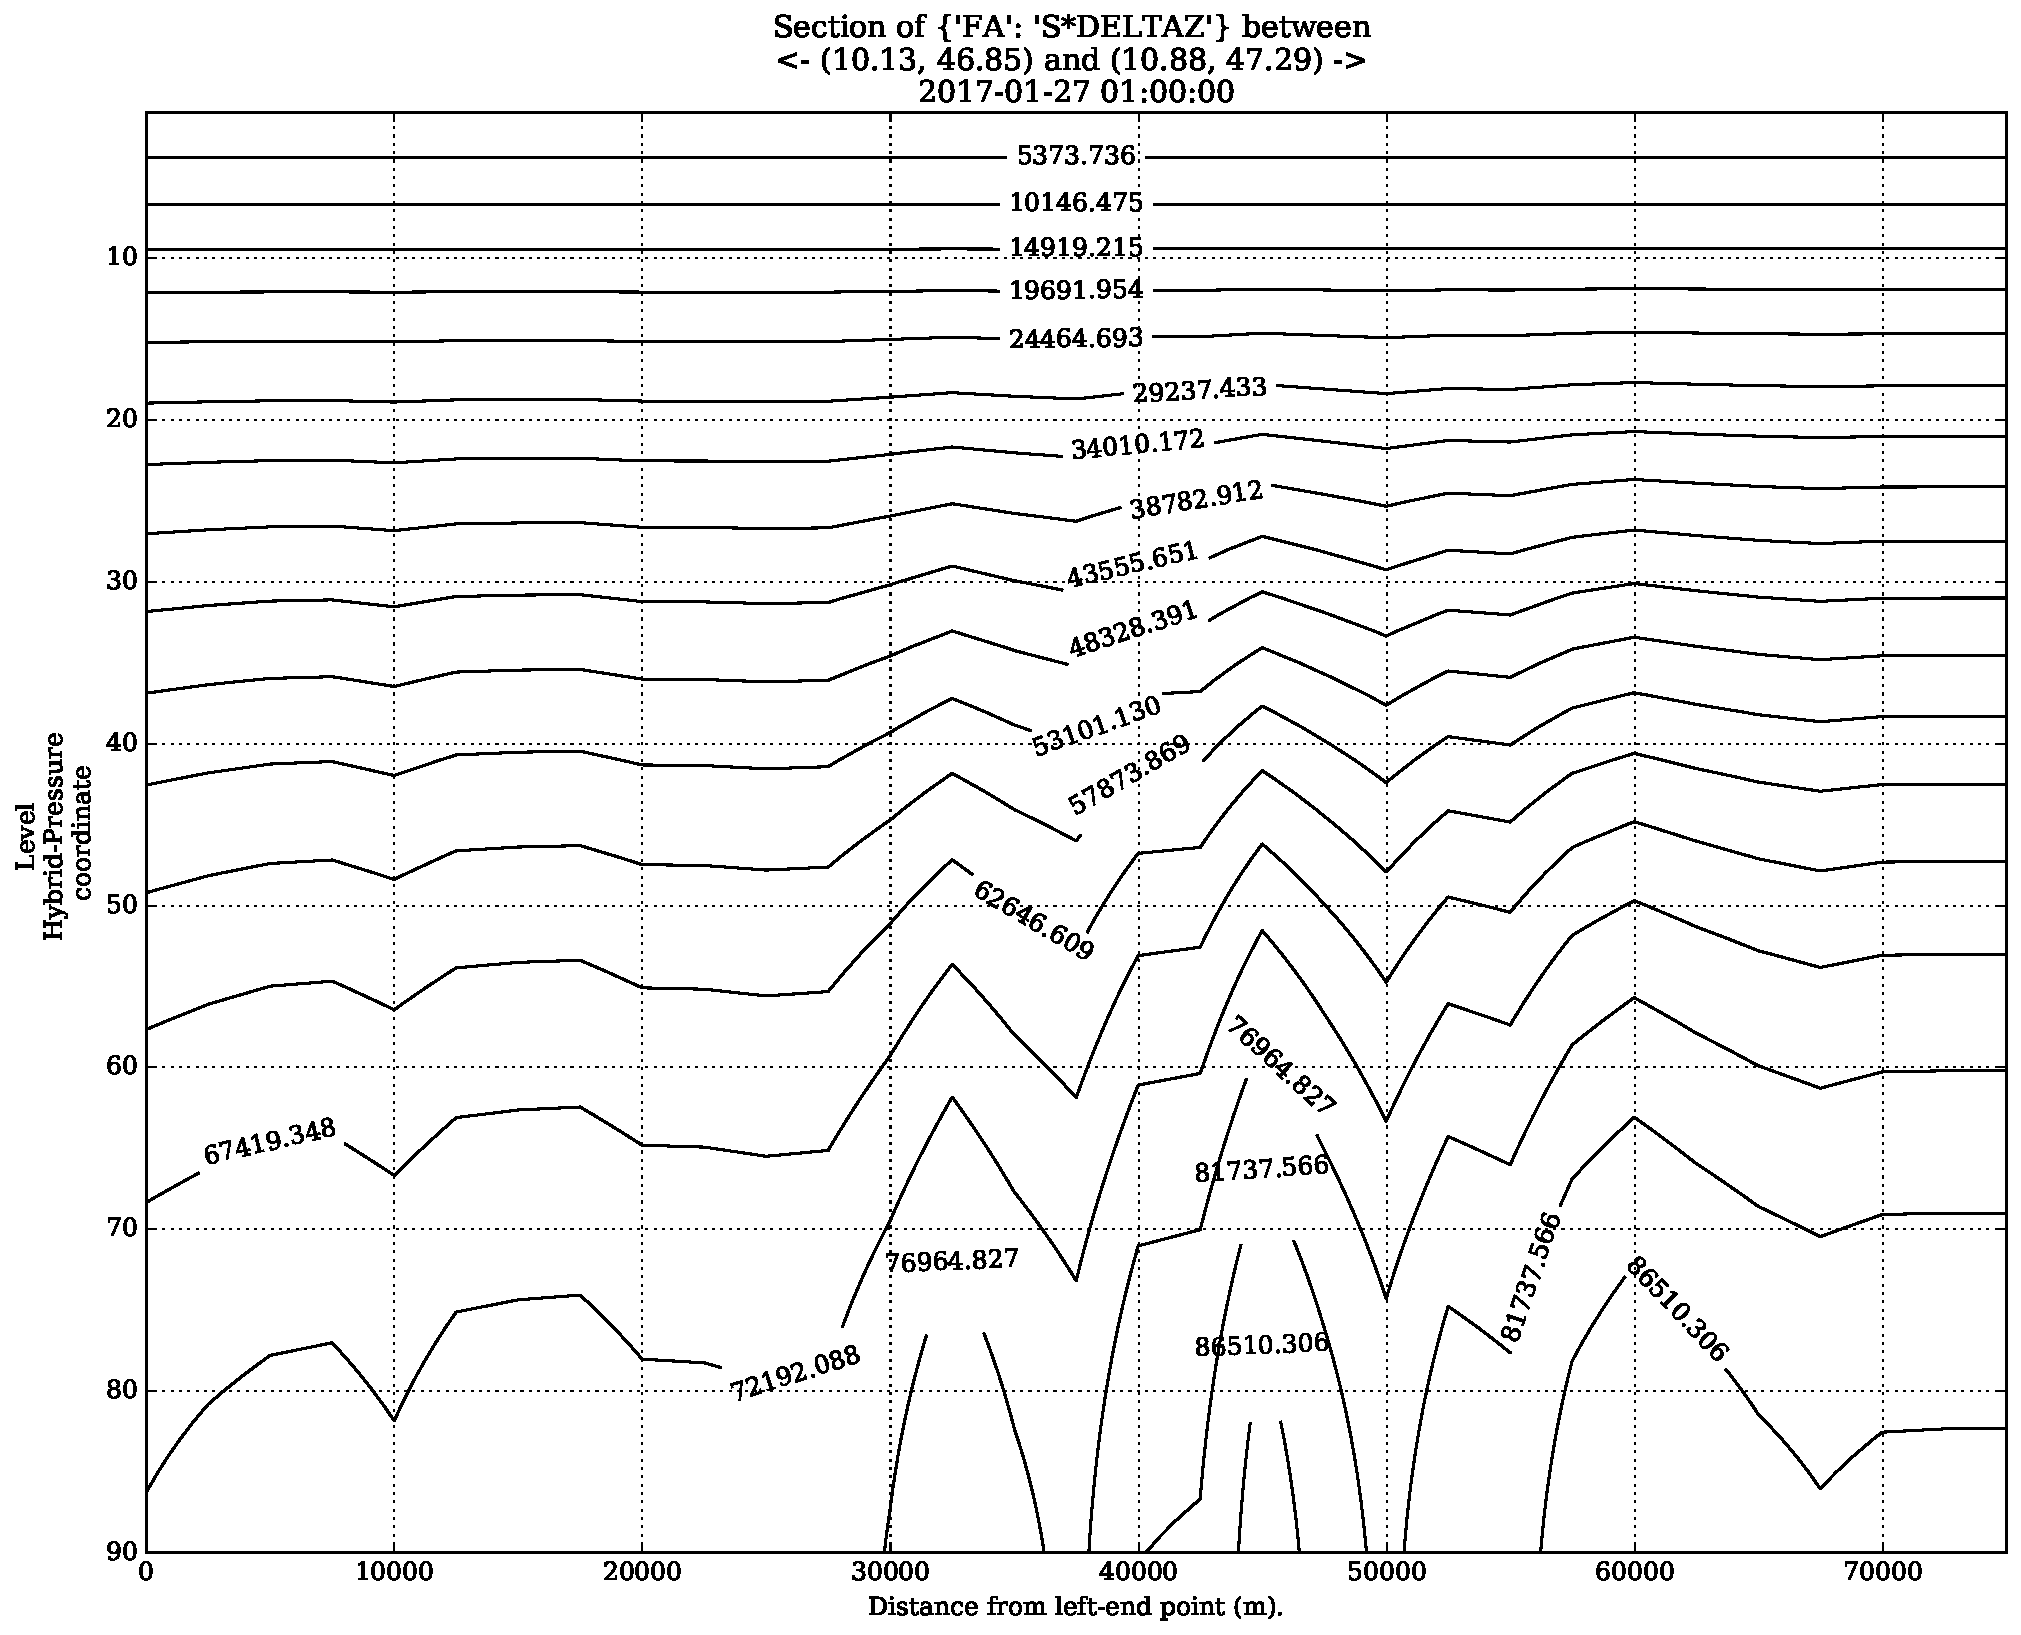
\includegraphics[trim={0cm 0cm  0cm  1.8cm },clip,width=\textwidth]{graphics/coordinates/PvsHybrid.pdf}
    \caption{\footnotesize{Hybrid Pressure-Terrain-following coordinates: layer number on Y-axis}}
    \label{fig:PvsHybrid}
    \end{subfigure}
    \hspace{1cm}
    \begin{subfigure}{0.45\textwidth}
    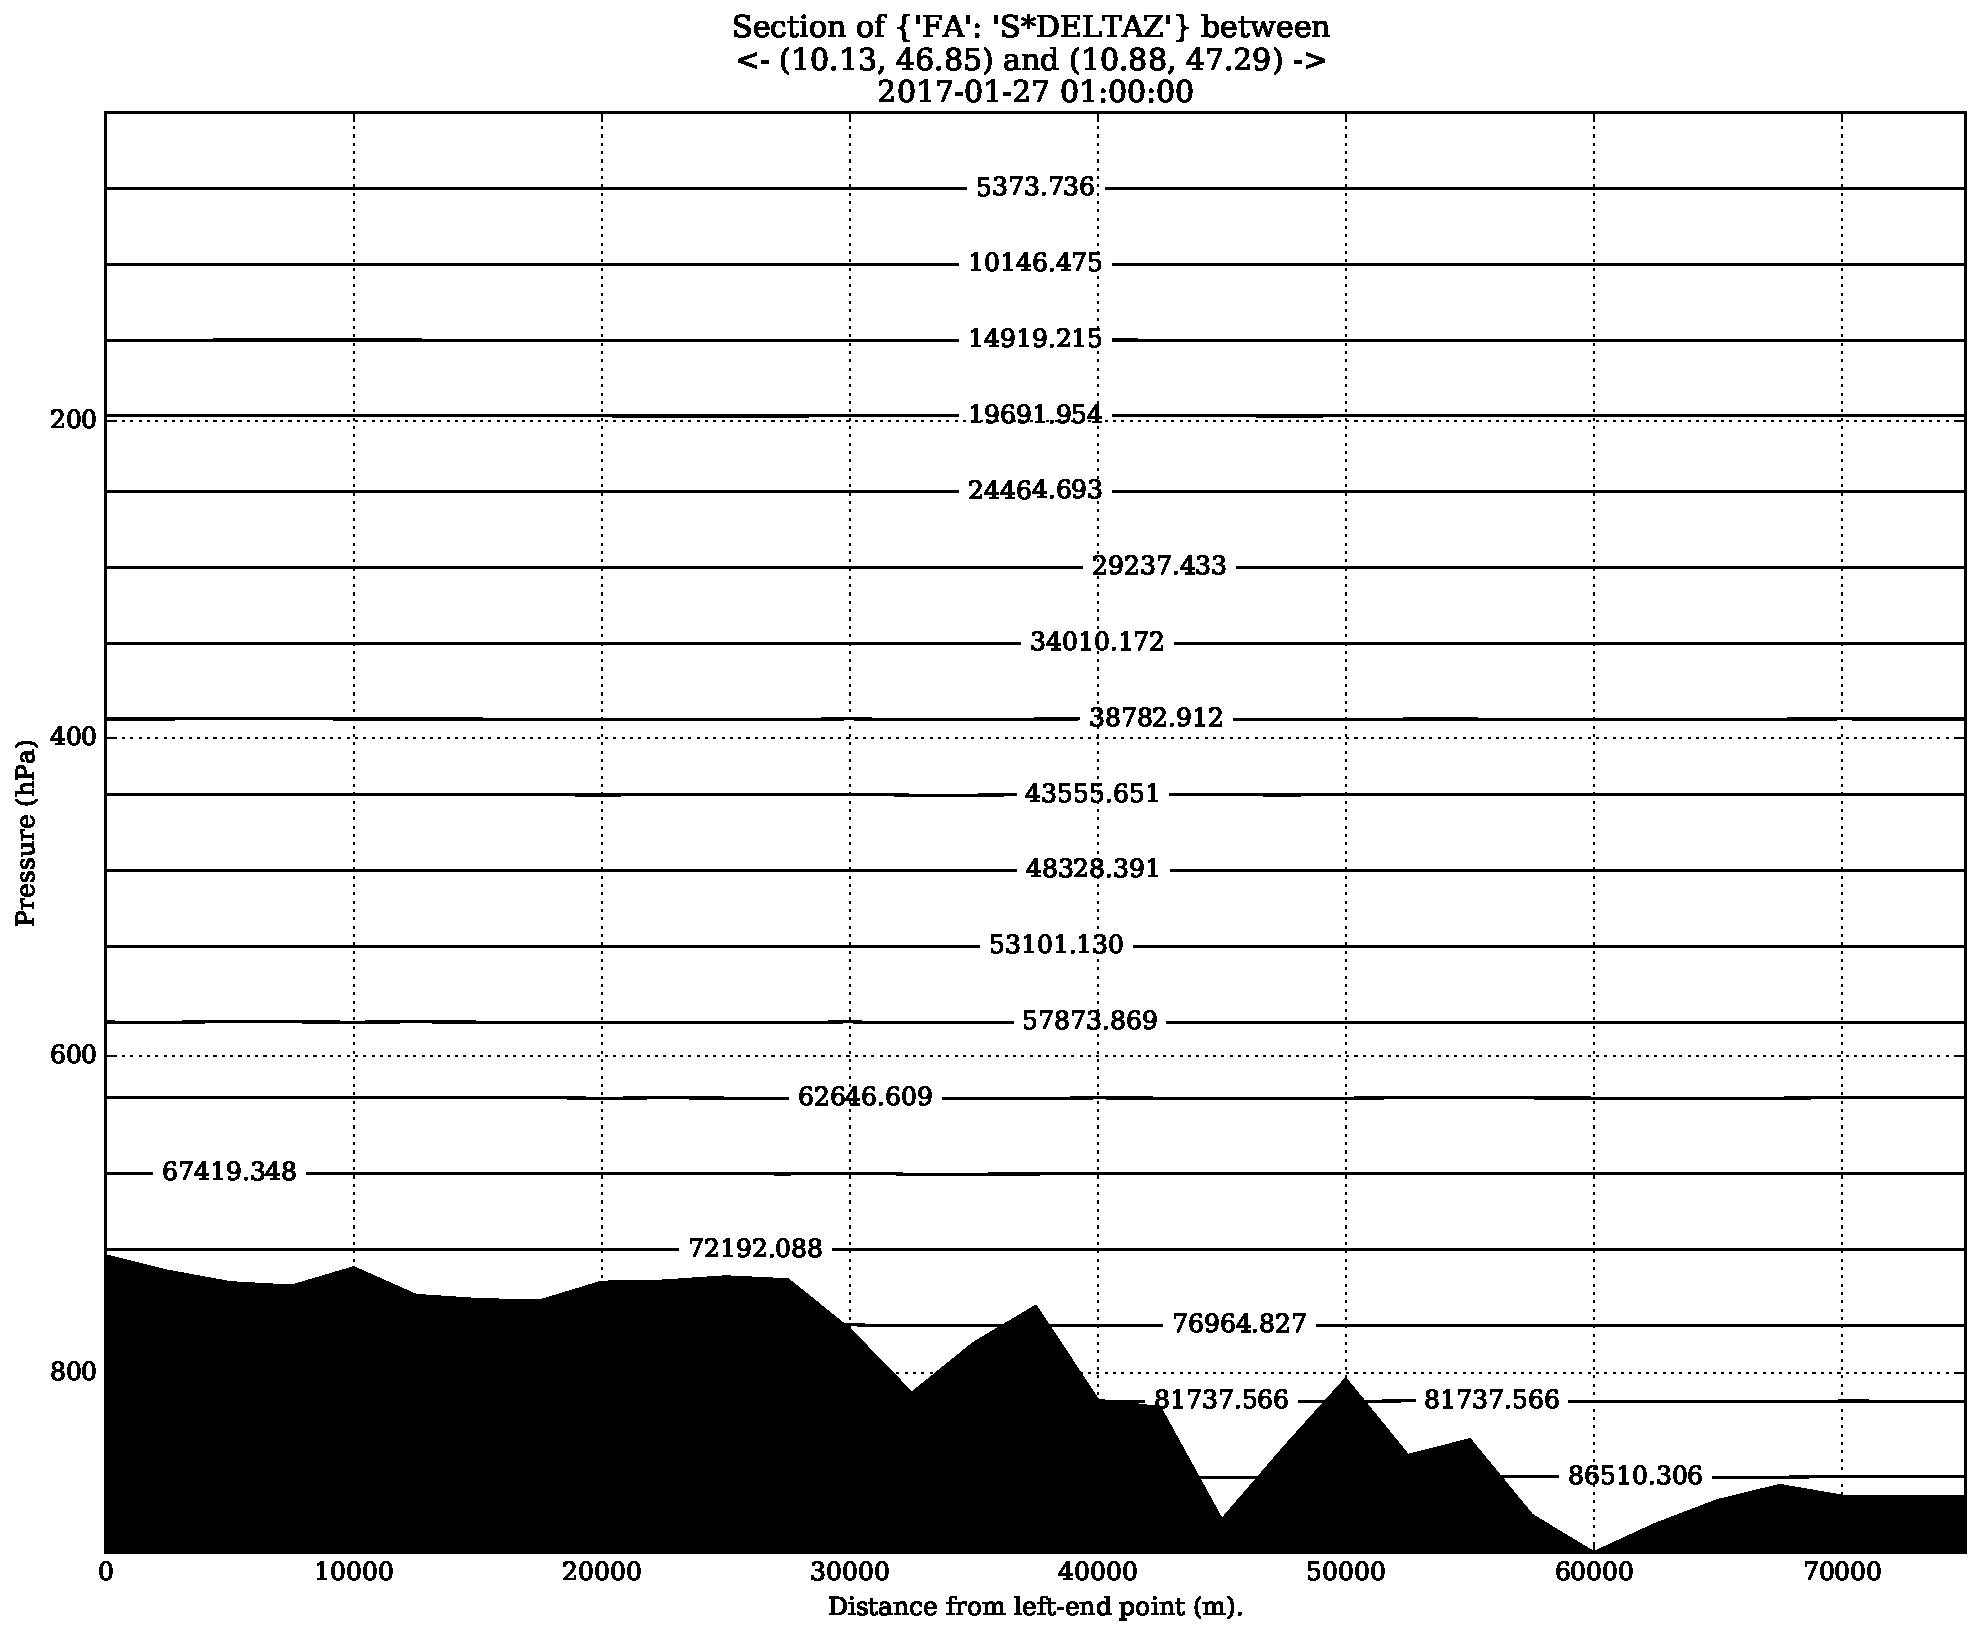
\includegraphics[trim={0cm 0cm  0cm  1.8cm },clip,width=\textwidth]{graphics/coordinates/PvsPressure.pdf}
    \caption{\footnotesize{Pressure coordinates: pressure [hPa] on Y-axis}}
    \label{fig:PvsP}
    \end{subfigure}
    \vspace{1cm}
    \begin{subfigure}{0.45\textwidth}
    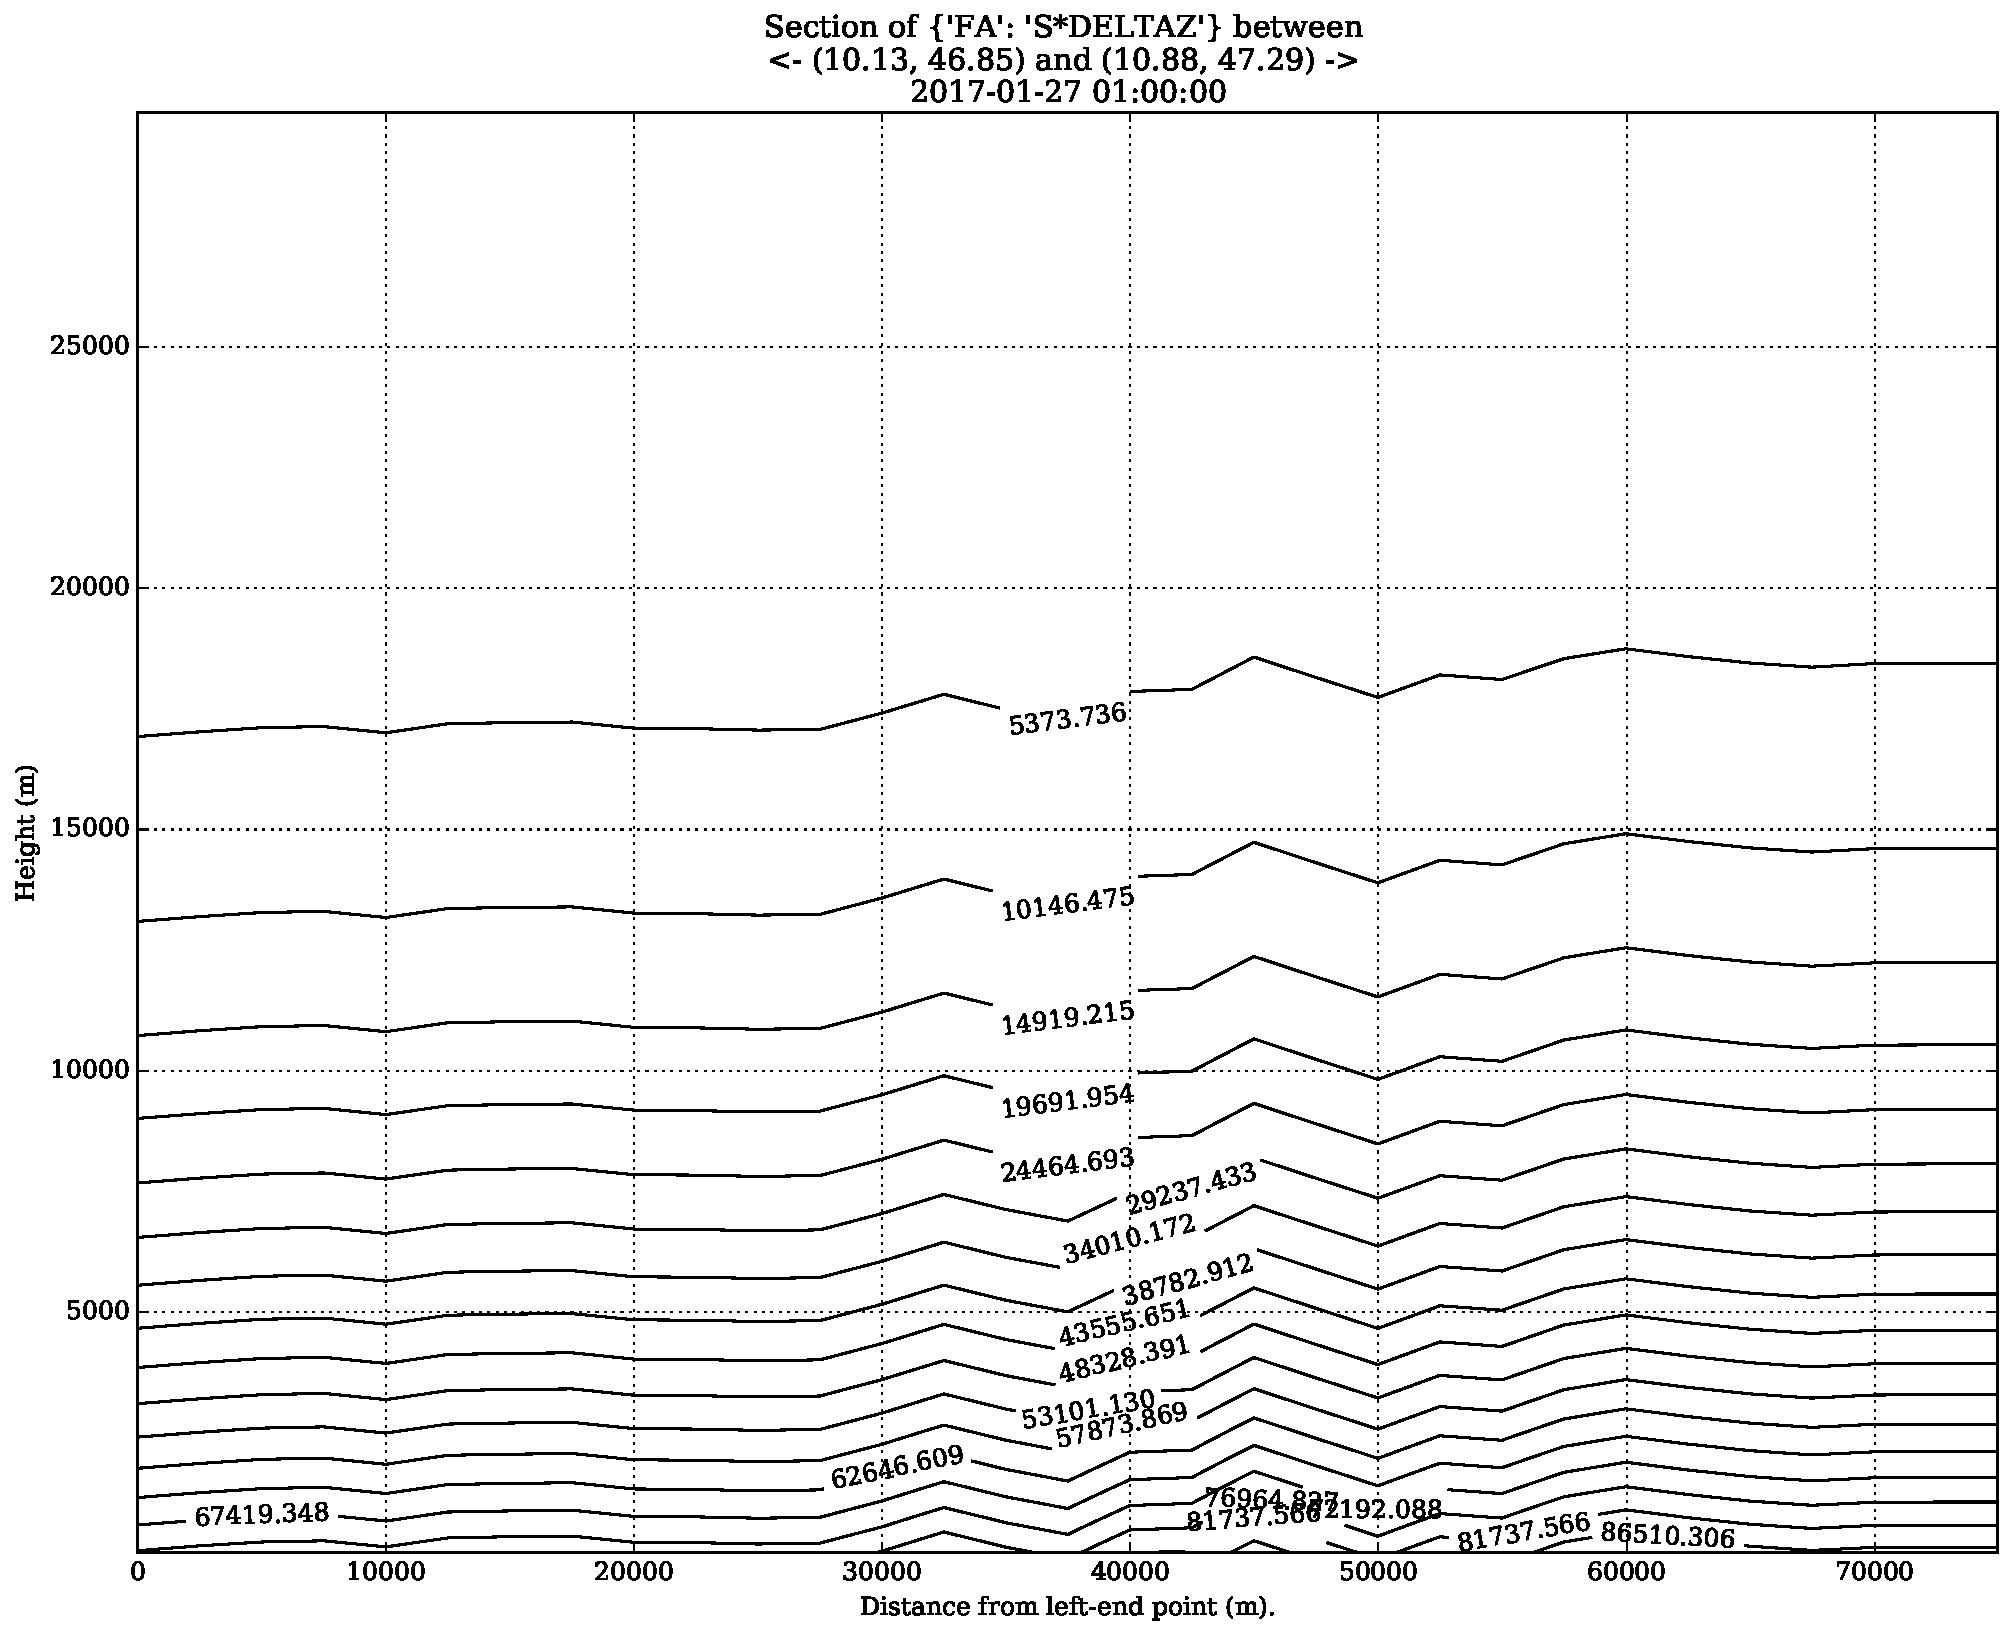
\includegraphics[trim={0cm 0cm  0cm  1.8cm },clip,width=\textwidth]{graphics/coordinates/PvsHeight.pdf}
    \caption{ \footnotesize{Terrain-following  coordinates: height above ground [m] on Y-axis}}
    \label{fig:PvsH}
    \end{subfigure}
    \hspace{1cm}
    \begin{subfigure}{0.45\textwidth}
    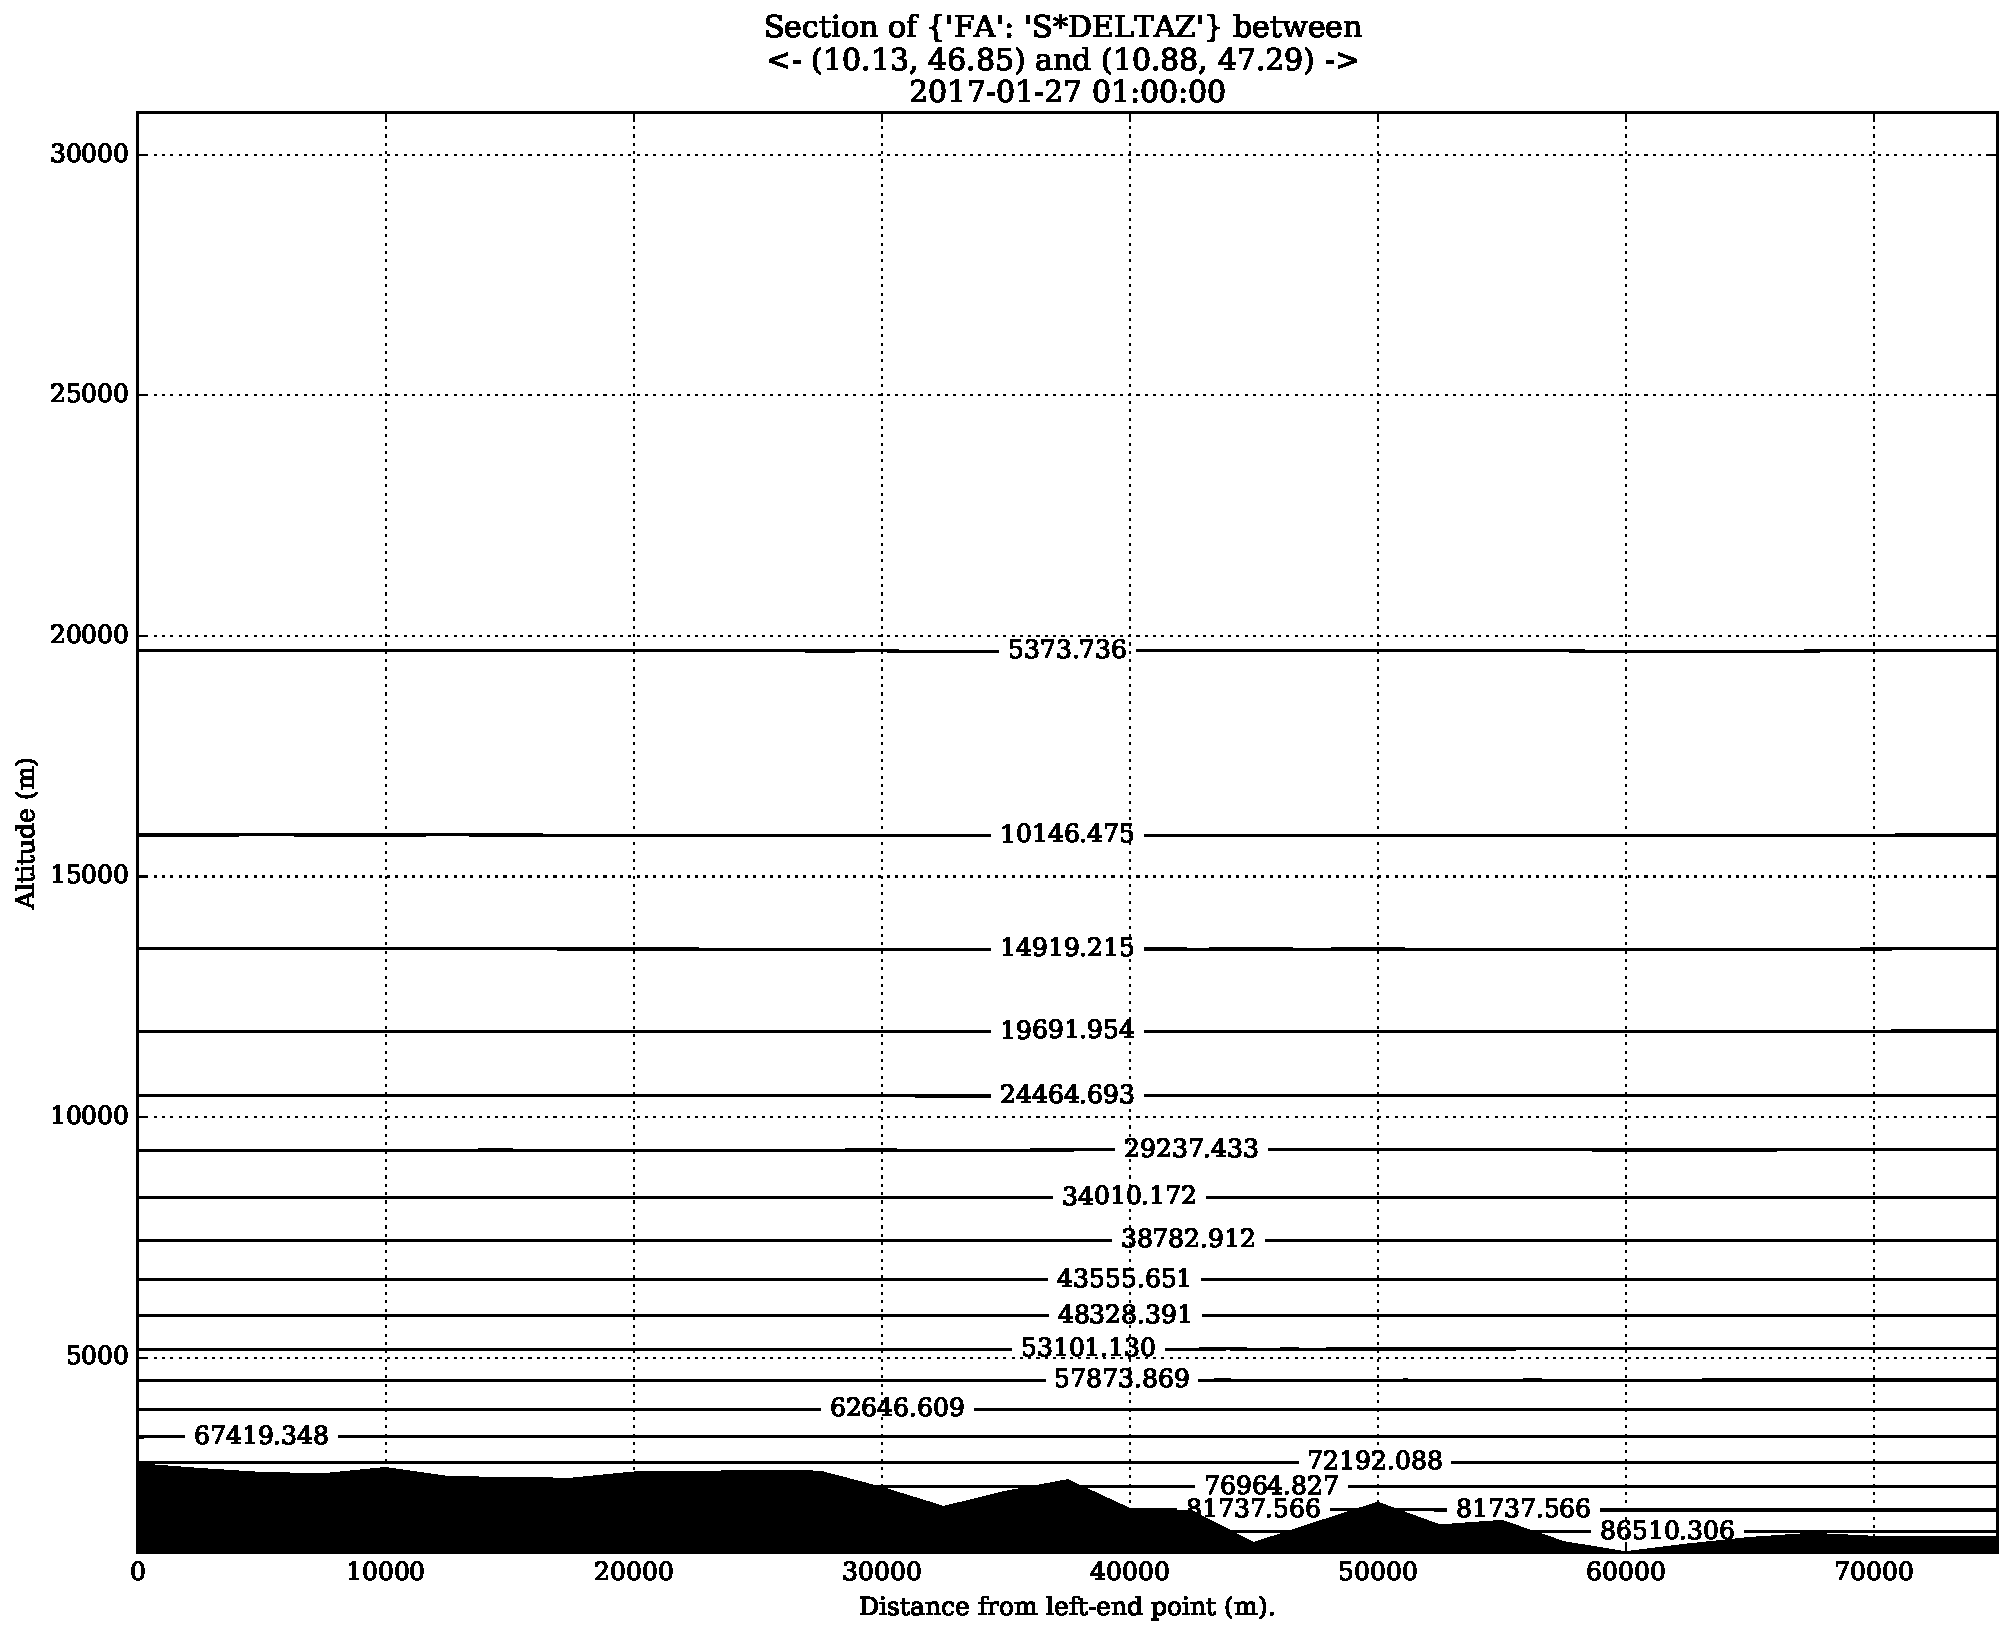
\includegraphics[trim={0cm 0cm  0cm  1.8cm },clip,width=\textwidth]{graphics/coordinates/PvsALtitude.pdf}
    \caption{\footnotesize{Traditional Height Coordinates: height above sea-level [m] on Y-axis}}
    \label{fig:PvsA}
    \end{subfigure}
    \caption[Comparison of Vertical Coordinate Systems]{Isobars in different vertical coordinate systems: 18 isobars (in [Pa]) of a cross section are shown in four different coordinate systems. The Y-axis is the vertical coordinate, different in each plot, and the X-axis is the horizontal distance from the starting point of the cross section. The cross sections starts at [lon:10.13, lat:46.85] (left end)  and ends at [lon:10.88, lat:47.29], showing a part of the Alps in western Austria to illustrate how topography is represented in different coordinate systems. Topological structures that cannot be a value assigned to are indicated as black surface.}
    \label{fig:coordinates}
\end{figure}
%draw simple figure to illustrate difference

\begin{figure}[p]
    \centering
    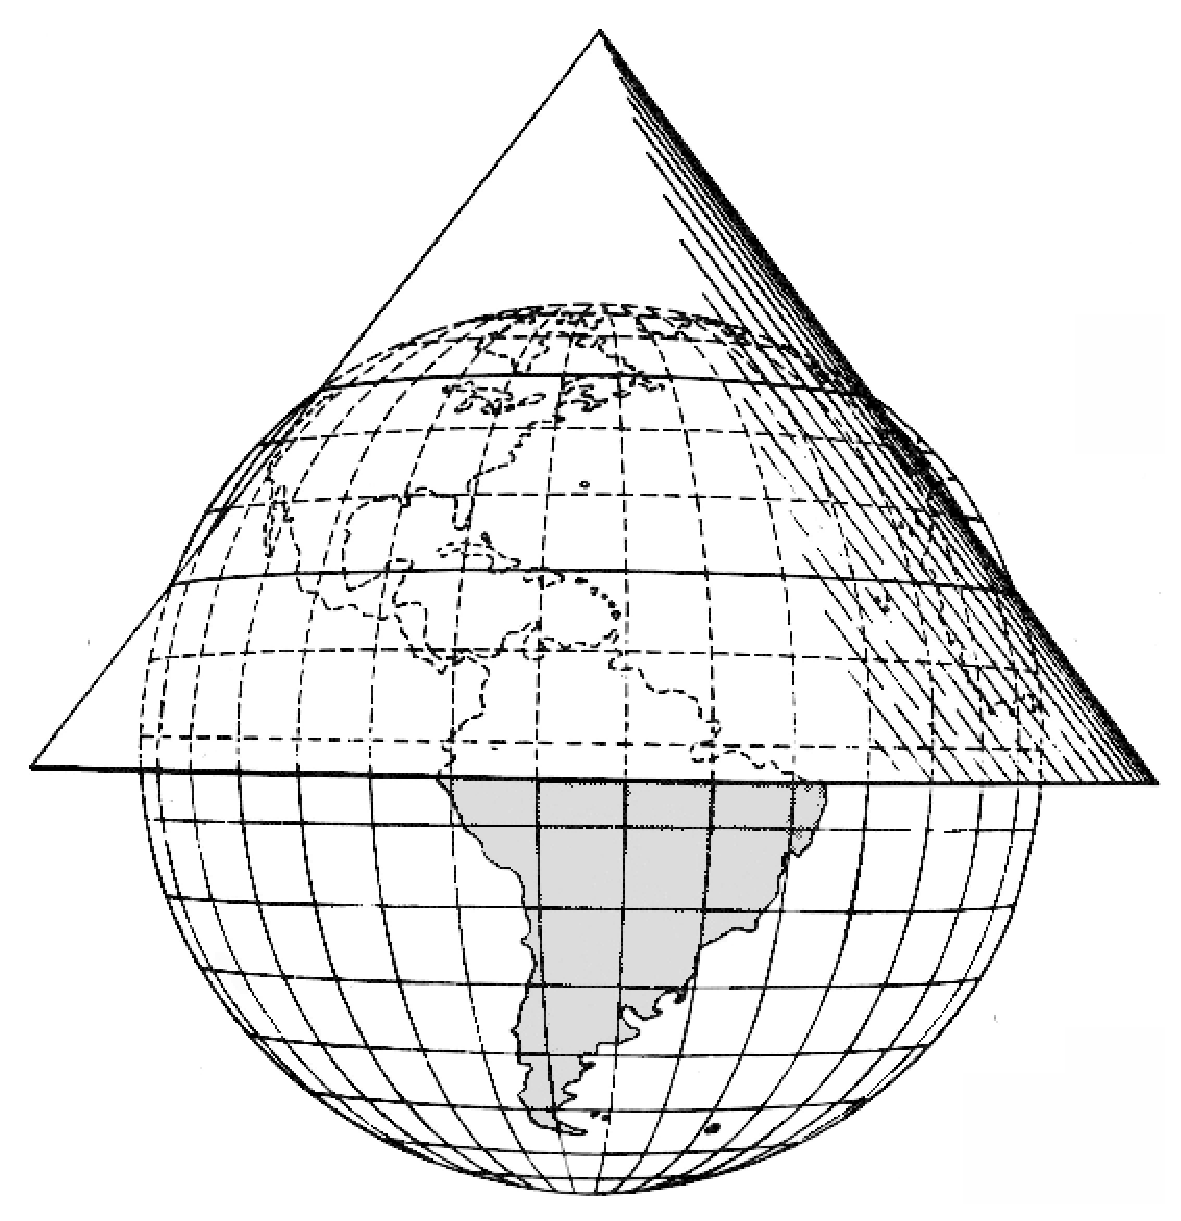
\includegraphics[width=\textwidth]{graphics/Lambert.eps}
    \caption[Lambert Projection]{Illustration of a conic conformal Lambert projection. Image by \citeauthor{usgs} \cite{usgs}}
    \label{fig:lambert}
\end{figure}
\newpage
\section{Pattern Generator}
\label{sec:pattern gen}
To perform Monte-Carlo forecasts by creating a stochastic physics ensemble a random number generator is needed. In most cases spatially and/or temporal correlations are necessary to represent realistic deviations from the deterministic scenario. To do so, a pattern generator that provides suitable randomly sampled spatial and temporal patterns, which can be applied to the relevant fields in the model, is the tool of choice.
In the AROME model the stochastic pattern generator generates a two-dimensional pattern, where the points are sampled from a normal distribution. Since the ranges of the quantities we want to perturb are restricted, the ranges of the perturbations need to be restricted as well.
Therefore a so-called clip ratio $x_{\mathrm{clip}}$ is defined in the namelist. Then, as described in the following by Equation \eqref{eq:fouriercoeff}, the distribution is cut off at the value of $x_{\mathrm{clip}}$ times the standard deviation $\sigma_{\mathrm{2D}}$. In this case `cut off' means, that if we define $a=x_{\mathrm{clip}} \sigma_{\mathrm{2D}}$, all sampled values outside the interval $[ -a, a] $ are set to $-a$ or respectively $a$.
This leads to the undesired result that the probability density function $f(p)$ does not have its minima, as desired at the edge of the mathematical domain. In fact, if the value for  $\sigma_{\mathrm{2D}}$ is too small, it can happen that the $f(p)$ has its maxima at the edges of the interval.

Another problem is that the pattern generator can only produce normal distributions. If the variable is suspected to be distributed differently, the only way to construct other distributions of randomly sampled numbers, is by use of the normally distributed pattern (e.g. taking the exponential of the numbers for lognormal distribution). Thus, one is severely limited in the selection of distribution. 

\subsection{Technical Set-Up of the Pattern Generator}

The pattern is constructed in spectral space and the corresponding coefficients $\hat{a}_{n,m}$, presented in Equation \eqref{eq:fouriercoeff}, are the coefficients of a double Fourier series. The pattern generator was originally implemented and described by \citeauthor{palmer2009stochastic} \cite{palmer2009stochastic} for the global ECMWF IFS model, where $\hat{a}_{n,m}$ relates to the spherical harmonics. The different coefficients are a consequence of the different representation of spectral fields in the ECMWF IFS and the AROME model. When the pattern generator is used on a LAM model the statistical properties of the fields are conserved, but the LAM fields are not congruent with the LAM domain of the global fields.\\
The spectral coefficients are obtained by random sampling and evolved by an auto-regressive process as described in Equation \eqref{eq:fouriercoeff}. 
\begin{equation}
\label{eq:fouriercoeff}
    \hat{a}_{n,m}(t+ \Delta t)= \Phi_{t} (t) \hat{a}_{n,m} +\sigma_{\mathrm{2D}}(n) \epsilon_{m,n} \Theta(x_{\mathrm{clip}}-\epsilon_{m,n})\Theta(\epsilon_{m,n} -x_{\mathrm{clip}})
\end{equation}
\begin{align*}
    \epsilon_{m,n} \in \mathbb{C}: \ 
 \Re(\epsilon_{m,n}) 
\sim N_{1}( \mu=0, \sigma=1); \  \
\Im(\epsilon_{m,n})
\sim N_{2}( \mu=0, \sigma=1)
\end{align*}

Here $ \Theta$ denotes the Heaviside step function which is defined as: 
\begin{flalign*}
&\Theta : \mathbb{R} \rightarrow \{ 0,1 \} \\
&x < 0: \Theta(x) = 0\\
&x \geq 0 : \Theta(x) =1\\ \quad .
\end{flalign*}
The random number generator samples the real and the imaginary part of  $\epsilon_{m,n}$ independently from a Gaussian distribution with variance $\sigma=1$ and mean $\mu=0$. $\epsilon_{m,n}$ is sampled independently for each $ m,n$ and $t$, where $n$ is the total wave number and $m$ is the zonal wave number, as defined in Equation \eqref{eq:zonalwavenumber}. The zonal wave number is the wave number for periodic boundary conditions at a given latitude $\phi$
\begin{equation}
m \lambda=2 \pi R_{\mathrm{E}} cos(\phi) \quad ,
\label{eq:zonalwavenumber}
\end{equation}

where $R_{\mathrm{E}}$ is the Earth's radius, $\phi$ the latitude and $\lambda$ the wavelength. Then the sample gets cut off below and above the clip ratio  $x_{\mathrm{clip}}$  and scaled by $\sigma_{\mathrm{2D}}(n)$.



Each  pattern $\Psi$ is characterized by its spatial correlation $ L_{\Psi}$ and its temporal correlation $ \tau_{\Psi}$, because those two parameters determine $\Phi_{\mathrm{t}} (t)$ and $\sigma_{\mathrm{2D}}(n)$ which define the spectral coefficients of the pattern, as demonstrated by Equation \eqref{eq:fouriercoeff}. The dependencies of  $\Phi_{t} (t)$ and $\sigma_{\mathrm{2D}}(n)$ on the correlation scales are non-linear and defined as the following:\\
\begin{equation}
    \Phi_{t} = \exp \left( \frac{ - \Delta t}{\tau_{ \Psi}} \right)
\end{equation}
\begin{equation}
    \sigma_{\mathrm{2D}}(n) = F_{0} \ \chi(n)
    \label{eq:std}
\end{equation}
\begin{equation}
    F_{0}=\frac{\sqrt{1 - \Phi_{t}^2} \ \sigma_{\mathrm{nl}}}{ \gamma}  
\end{equation}
\begin{equation}
    \chi =  \exp (-0.5 \  \zeta \  n \ (n+1))
\end{equation}
\begin{equation}
\zeta = 0.5 \left( \frac{L_{\Psi}}{R_{\mathrm{E}}} \right)^{2}
\end{equation}
\begin{equation}
    \gamma = \sum_{n} \sqrt{2n +1} \ \chi (n)
\end{equation}
The scaling parameters $\Phi_{t} (t)$, $ L_{\Psi}$, $x_{\mathrm{clip}}$ and $\sigma_{\mathrm{nl}}$ (relates to the variance of the distribution) are all set in the model configuration, called namelist hereafter.
\begin{figure}[h]
\captionsetup{width=.7\linewidth}
    \centering
    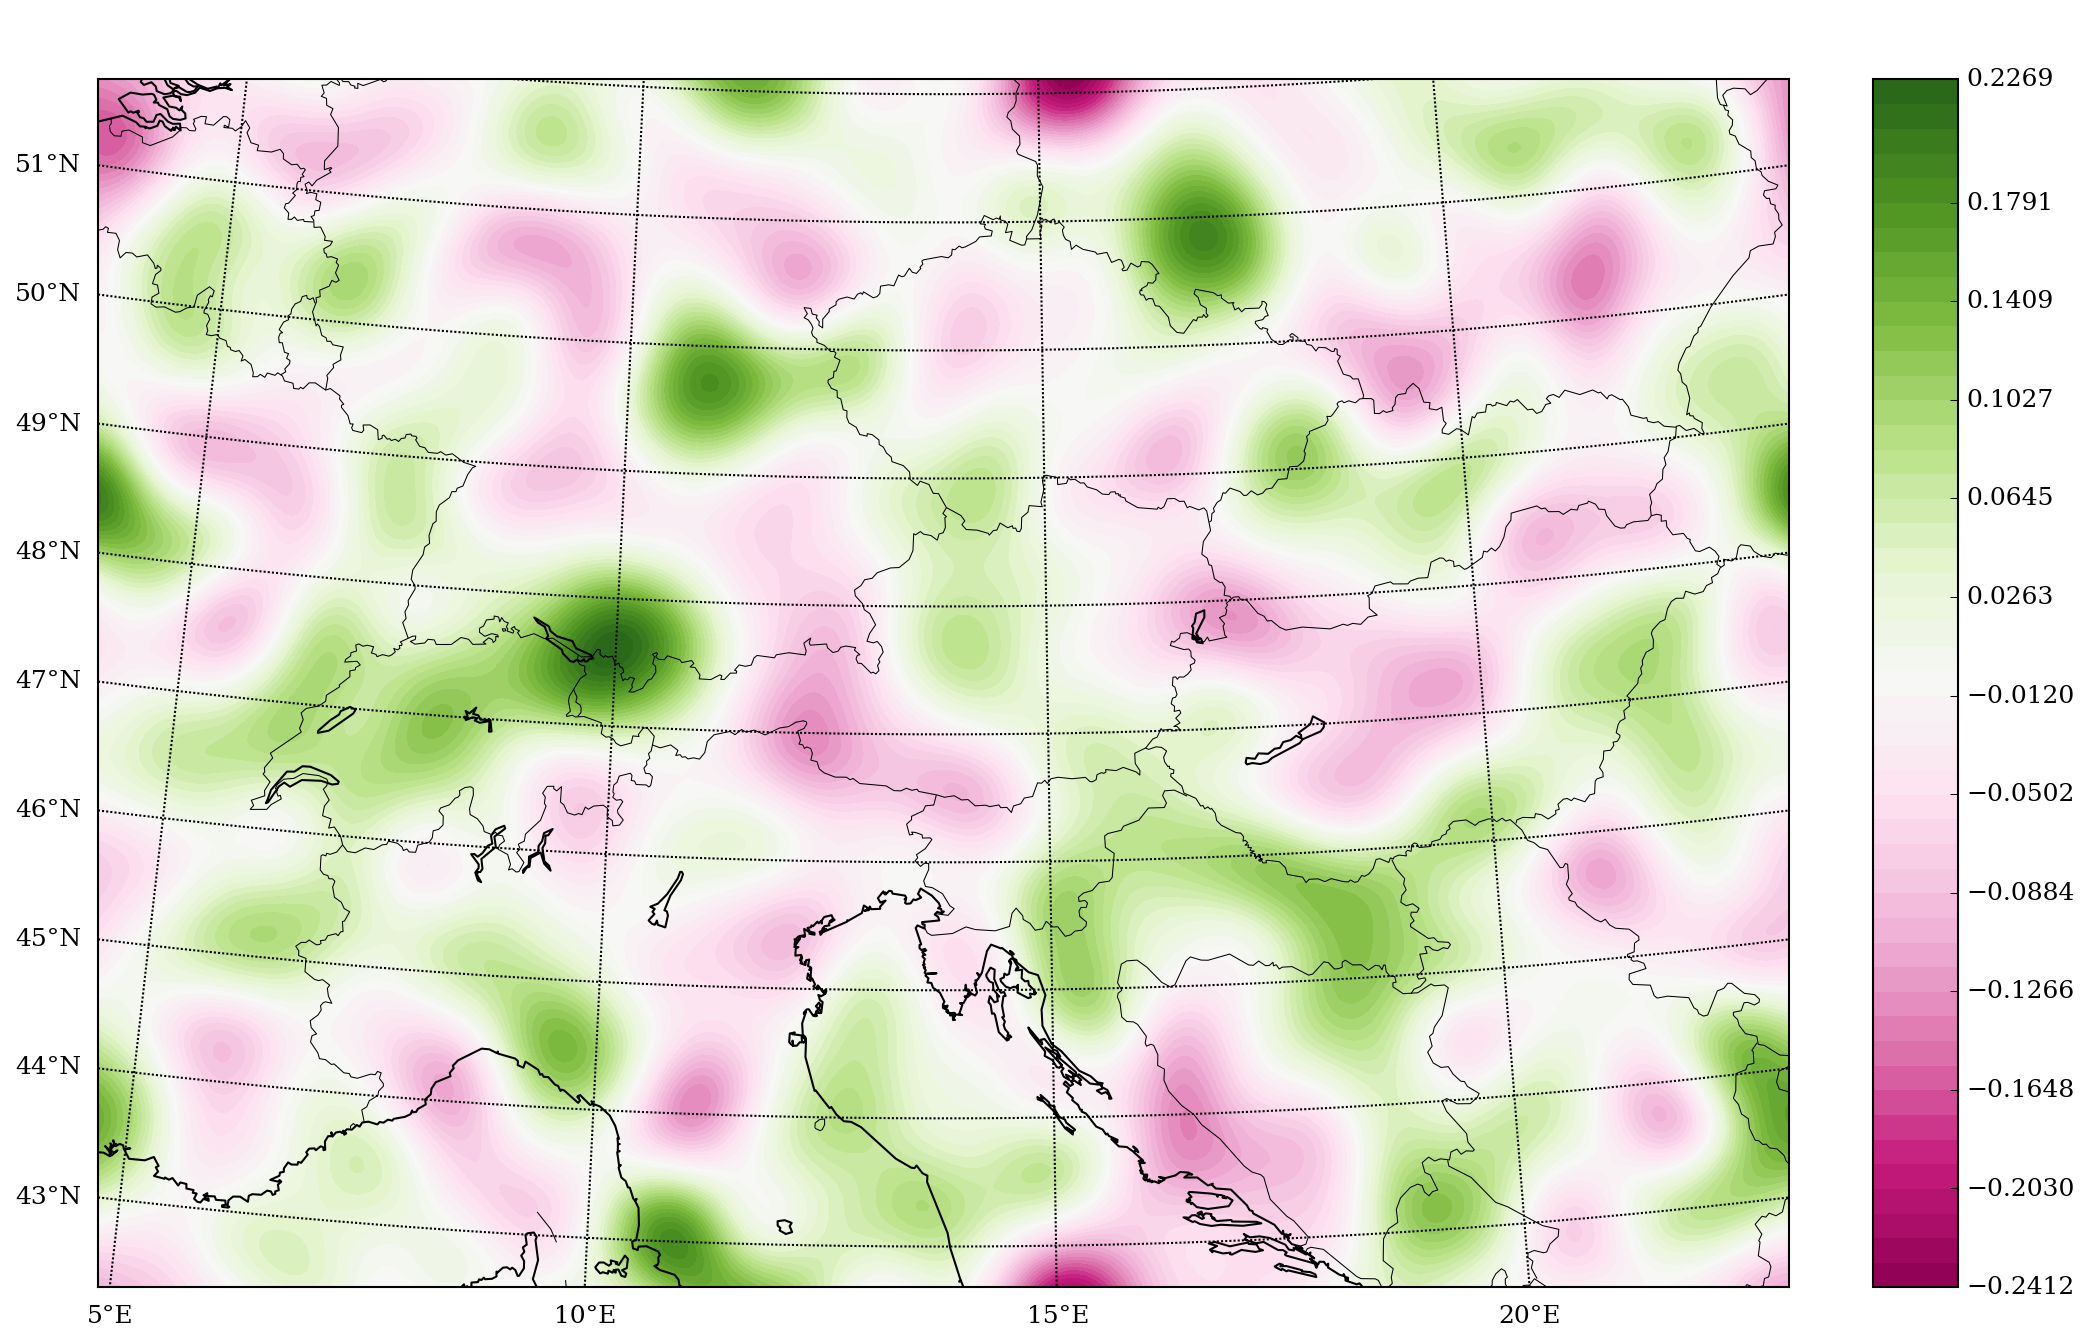
\includegraphics[width=0.7\textwidth]{graphics/mesoscale-pert.png}
    \caption[Example of a Small-Scale Perturbation]{Example of a normally distributed small-scale perturbation generated by the pattern generator}
    \label{fig:example-pert}
\end{figure}
